\FloatBarrier
\section{Baseline Model on Sequential Benchmark (Sequential, Homogeneous Dimension)}
We now outline the performance of the baseline model on the sequential benchmark, in a homogeneous-dimension setting, using ten queries from the same dimension (all colors, all shapes, or all textures). This setting is in contrast to the control setting we will describe next, in which we introduce a mixture of tasks from all three dimensions, which we term the sequential, heterogeneous dimensions setting. We will begin by providing a plot closer to the raw results, where we plot the model’s performance on the first task introduced, which it is restrained on ten times, and on each of the tasks during the episode in which it is introduced. Afterward, we will present more heavily processed representations of the results, which we devised in order to help evaluate how learning scales with training and how much catastrophic interference the model exhibits through the training on this sequential benchmark. 

Figure \ref{fig:results-baseline-sequential-raw-accuracy} offers a fairly unprocessed presentation of the performance of the baseline model in this setting. The results summarize six replications of the Latin square design detailed above for each dimension, for a total of sixty iterations through the benchmark in each dimension, or 180 combined. The top panel plots the course of the accuracy on the first task, for each of the ten times it was trained on during the benchmark. The color range used in this plot, from black to copper, will be used for every plot in which the individual trajectories vary by how many times the tasks in question were retrained. 
\begin{wrapfigure}{r}{0.5\linewidth}
\vspace{-.3in}
\begin{spacing}{1.0}
\centering
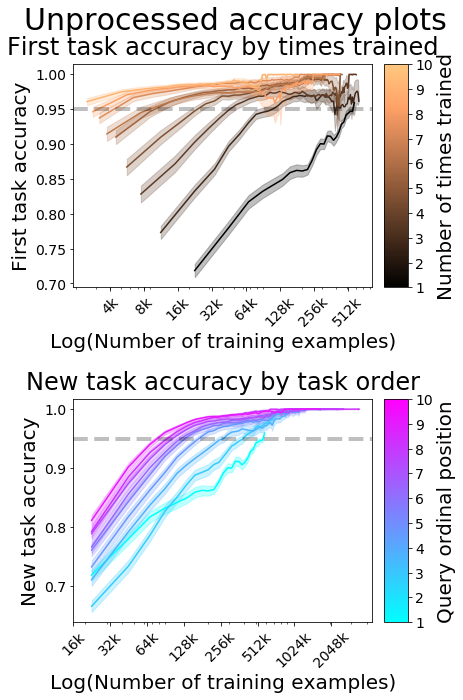
\includegraphics[width=0.95\linewidth]{ch-results/figures/baseline_sequential/unprocessed_accuracy.png}
\caption{ {\bf Unprocessed accuracy results.} Using the baseline model in the sequential, homogeneous dimensions condition. \textbf{Top:} First task accuracy by number of times trained. \textbf{Bottom:} New-task accuracy by order presented to the model. }
\label{fig:results-baseline-sequential-unprocessed-accuracy}
\end{spacing}
% \vspace{-.25in}
\end{wrapfigure}
The curves originate from different points as the number of examples per episode allocated to the first task change, from 22,500 in the first episode until 2500 in the last one. Note that the model substantially improves as it retrains on this task additional times; we will revisit this result. The bottom panel plots the accuracy of the new task in every episode. The color range used in this plot, from teal to pink, will be used for every plot in which the individual trajectories vary by which query in the order they represent. These plots all originate at the same x-value (of 22,500) since the newest task always receives 22,500 examples per epoch. This plot also shows the model improving as training proceeds, with later tasks originating at higher accuracy and reaching the threshold faster.

\begin{figure}[!htb]
% \vspace{-0.225in}
\centering
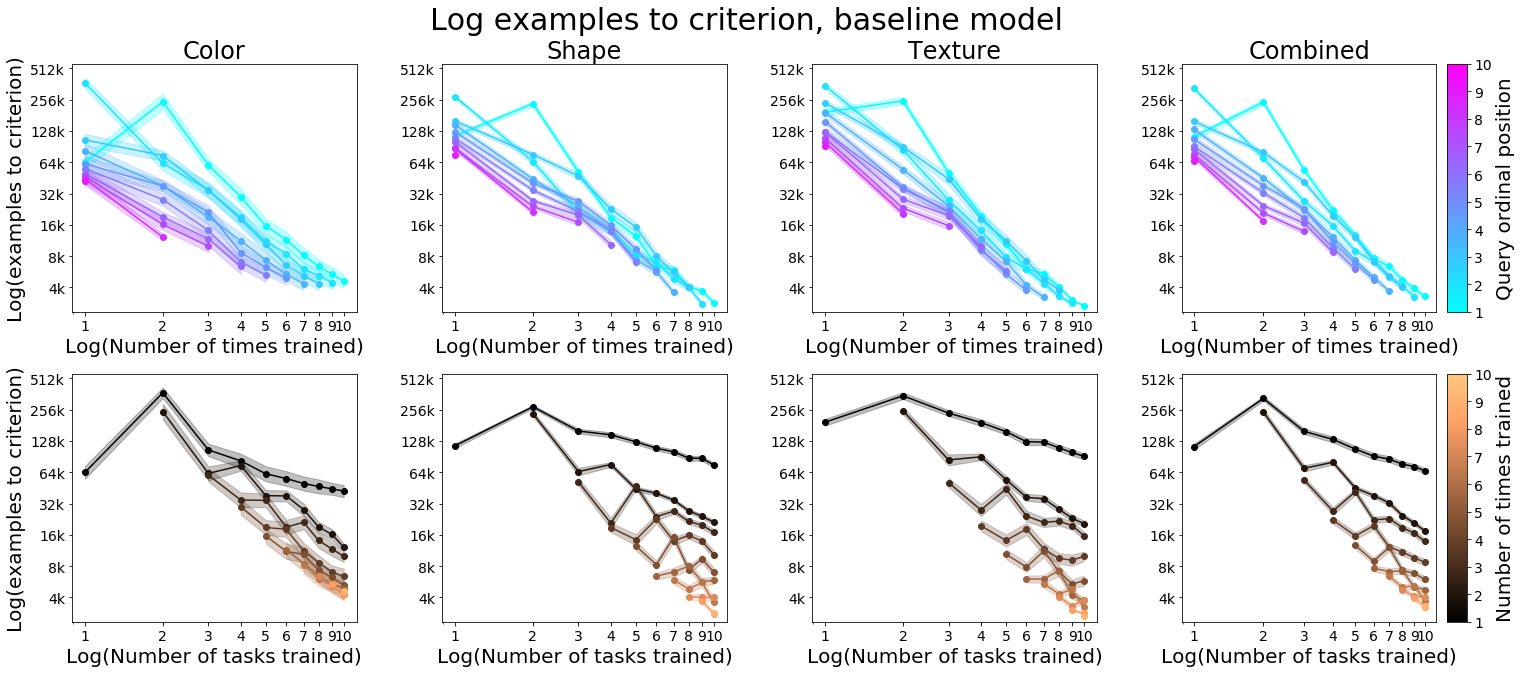
\includegraphics[width=\linewidth]{ch-results/figures/baseline_sequential/examples_to_criterion.png}
\caption{ {\bf Log examples to criterion.} Using the baseline model in the sequential, homogeneous dimensions condition. Both panels use a log-log scale, and in both plots the shaded region represents the standard error of the mean (SEM). \textbf{Top:} Plotted by number of times trained. Color scales from first task presented (brightest blue) to last task (cyan) \textbf{Bottom:} Plotted by number of tasks currently trained. Color scales from the first time a task was trained (black) to the tenth time a task was trained (copper).}
\label{fig:results-baseline-sequential-examples-to-criterion}
% \vspace{-0.2in}
\end{figure}

Figure \ref{fig:results-baseline-sequential-examples-to-criterion} depicts the performance of the baseline model in a different form, which helps us visibly examine the scaling behavior as the model proceeds through the task. We plot the performance in the iterations for each dimension alone, as well as combined. Each iteration through the benchmark contributes fifty-five data points: the first task introduced was trained on ten times, the second task nine times, the third task eight times, and so forth until the last task, which was only trained on once. We then average the performance on a particular metric, in this plot the log of the number of examples required to reach the accuracy criterion, over all iterations for each of the fifty-five data points. This process results in the average of the log of the number of examples to reach criterion based on (a) which ordinal position a task occupied in an iteration through the benchmark and (b) how many times it was previously trained on within that iteration. 

The top panels show the scaling behavior, as the log of the number of examples required to reach criterion, by the number of times each task was trained on. As above, each color on the spectrum marks a specific task in the order, from the first task introduced in cyan to the last one in pink. We see linear scaling-behavior in the log-log scale, which indicates a power law behavior. All tasks require monotonically decreasing amounts of training for subsequent tasks, save for the second training on the first task introduced. One hypothesis to explain this observation is that the model somehow learns a fairly naive solution for the first task and that introducing subsequent tasks forces the model to learn better representations, which requires additional training. This interpretation is supported by the fact that the first time training the first task requires fewer examples than the first time on the third and fourth tasks (beyond just the second one). This behavior could be interpreted as further evidence for the naivety of the solution learned for the first task, compared to later learning more robust representations that support additional tasks. Otherwise, the behavior is remarkably consistent, where every additional time the model is trained on a task requiring fewer iterations, and each task showing better performance (as evidenced by a lower curve) than its predecessors. We interpret this result demonstrating that this naive model, with no explicit meta-learning capacity or a specialized architecture, shows a positive scaling behavior, and improves with each newly introduced task. 

The bottom panels offer a different perspective on the same data. Here we plot the same number of examples required to reach criterion, but by the total number of tasks the model is learning at each stage of the benchmark. Each color on the spectrum groups data points by the number of times a particular task has trained on; tasks trained on for the first time grouped in black, to tasks trained on the most time in copper color. We observe the same positive scaling outlined in the previous panels, where both later tasks and tasks trained on additional times require fewer examples to reach criterion. One unexplained anomaly in this plot is that for most groups, the third task in the group required more training than the second task in the group, as evidenced by the bump up in the third point in each colored line. We have no intuitive explanation for this result. 

Note that the individual dimensions qualitatively show the same behavior, even if scaled differently. While colors tend to be easier than shapes, which tend to be easier than textures, their profiles all appear sufficiently similar such that we will later only analyze the combined results, rather than belaboring over the individual dimensions. 

\begin{figure}[!htb]
% \vspace{-0.225in}
\centering
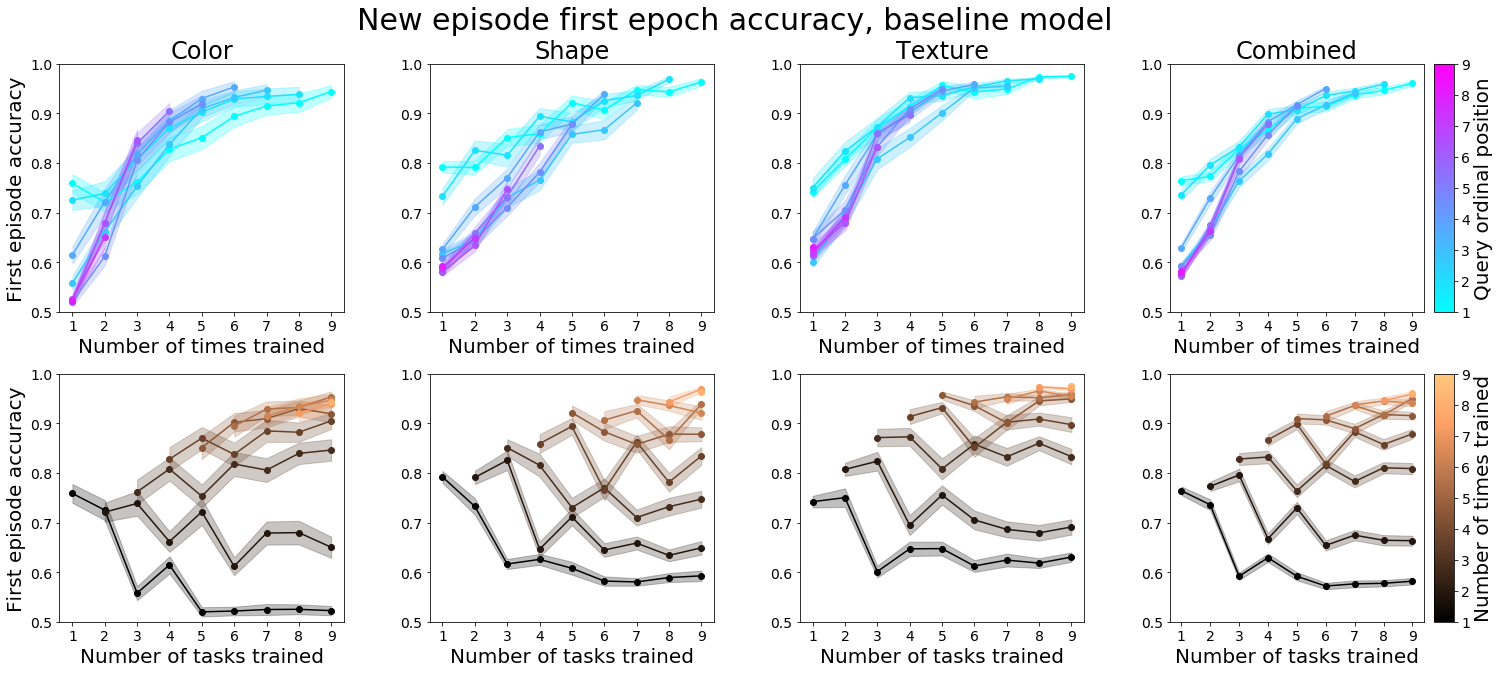
\includegraphics[width=\linewidth]{ch-results/figures/baseline_sequential/first_episode_accuracy.png}
\caption{ {\bf New episode first epoch accuracy.} Using the baseline model in the sequential, homogeneous dimensions condition. In both plots the shaded region represents the standard error of the mean (SEM). \textbf{Top:} Plotted by number of times trained. Color scales from first task presented (brightest blue) to last task (cyan) \textbf{Bottom:} Plotted by number of tasks currently trained. Color scales from the first time a task was trained (black) to the tenth time a task was trained (copper).}
\label{fig:results-baseline-sequential-first-episode-accuracy}
% \vspace{-0.2in}
\end{figure}

Figure \ref{fig:results-baseline-sequential-first-episode-accuracy} provides a measure of catastrophic forgetting organized similarly to Figure \ref{fig:results-baseline-sequential-examples-to-criterion}. We focus on the epochs introducing a new task to the model, in which we transition to a new episode. In other words, in the previous epoch, all current tasks reached the 95\% accuracy criterion on the held-out test set, and so on the current epoch, we transition episodes and introduce a new task. To measure forgetting, we examine the test-set accuracy on each task in after this first episode and examine how far it drops from its previous performance above 95\%. In this case, we have forty-five data points, rather than fifty-five, since we can examine the accuracy on the first task once every subsequent task is introduced, of which there are nine. Similarly, for the second task there are eight possible accuracy comparisons, and for the third task seven, and so forth, until we reach the last task introduced, for which we cannot compute this measure since none follow it.

The top panels depict, as before, this accuracy by the number of times a task was trained on. Tasks trained six times or more barely lose any accuracy, remaining above 90\% after the first episode with a new task. Forgetting, however, becomes worse as the model learns additional tasks -- while earlier tasks (in lighter blues) show an accuracy of around 75\% in their first time trained with new tasks, later tasks drop to around 60\%. The bottom panels again offer a different perspective on these same results. Here, we connect tasks by the number of times they have been trained on, and show a similar effect: after the first few tasks, the drop in the first new-task episode for later tasks is to an accuracy of around 60\%. We see the same third-repetition anomaly as before, where the drop for the third task in each of these groups is anomalous compared to the ones before and after it. 
